\documentclass{standalone}
\usepackage{tikz}
\usetikzlibrary{patterns, positioning}


\begin{document}
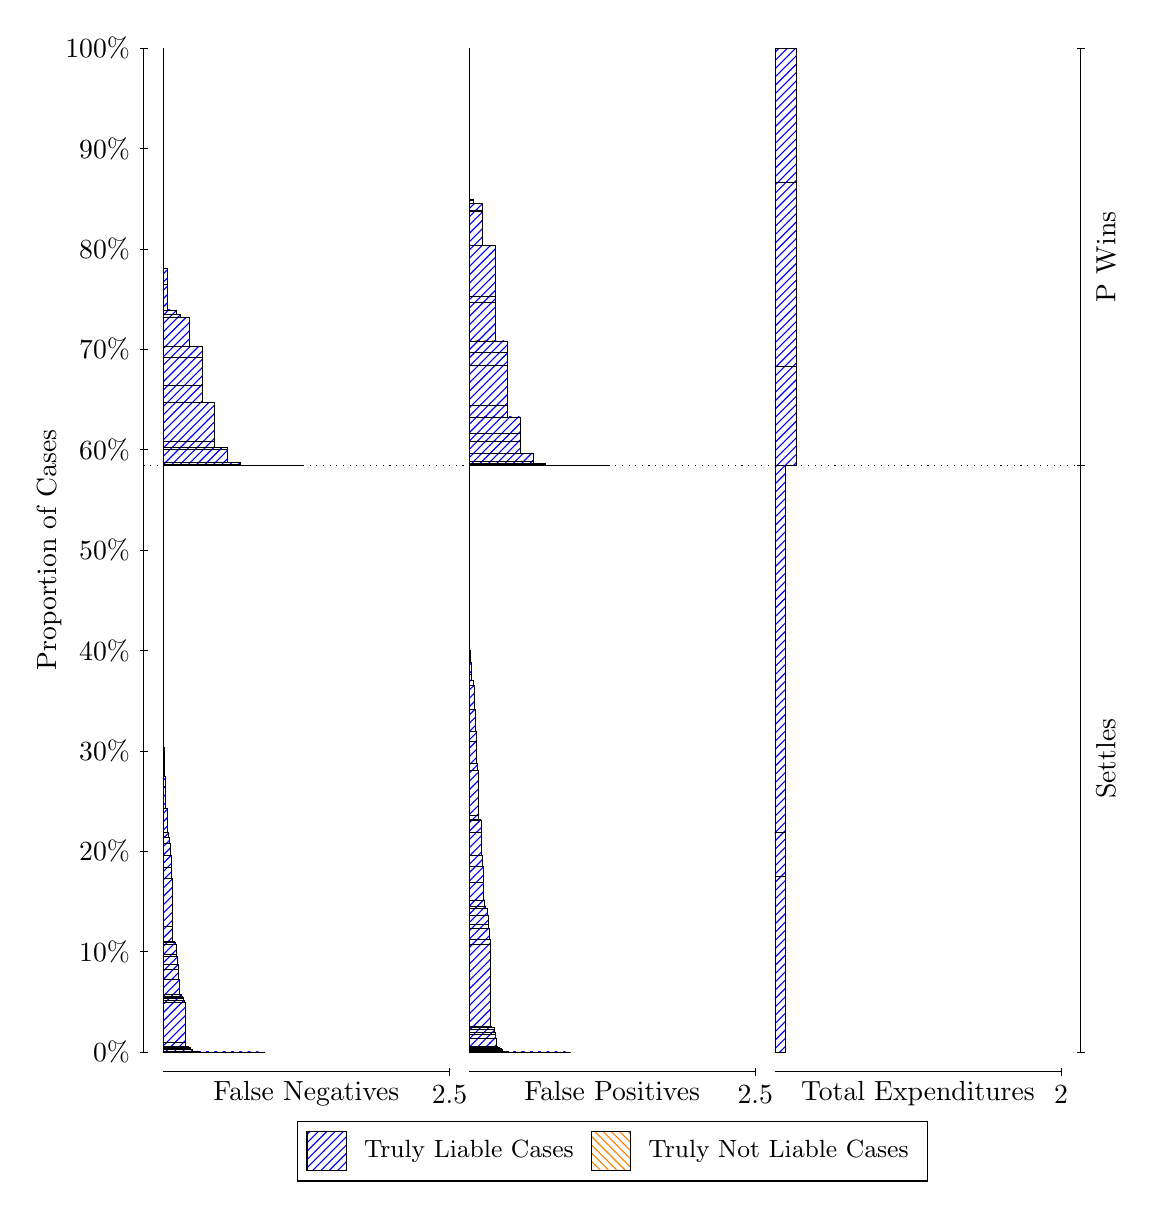
\begin{tikzpicture}
\draw[black, very thin] (1.5,1.75) -- (1.5,14.5);
\node[rotate=90, text=black, anchor=center] at (0.3, 8.125) {Proportion of Cases};
\draw[black, very thin] (1.45,1.75) -- (1.55,1.75);
\node[text=black, anchor=east] at (1.45, 1.75) {0\%};
\draw[black, very thin] (1.45,3.025) -- (1.55,3.025);
\node[text=black, anchor=east] at (1.45, 3.025) {10\%};
\draw[black, very thin] (1.45,4.3) -- (1.55,4.3);
\node[text=black, anchor=east] at (1.45, 4.3) {20\%};
\draw[black, very thin] (1.45,5.575) -- (1.55,5.575);
\node[text=black, anchor=east] at (1.45, 5.575) {30\%};
\draw[black, very thin] (1.45,6.85) -- (1.55,6.85);
\node[text=black, anchor=east] at (1.45, 6.85) {40\%};
\draw[black, very thin] (1.45,8.125) -- (1.55,8.125);
\node[text=black, anchor=east] at (1.45, 8.125) {50\%};
\draw[black, very thin] (1.45,9.4) -- (1.55,9.4);
\node[text=black, anchor=east] at (1.45, 9.4) {60\%};
\draw[black, very thin] (1.45,10.675) -- (1.55,10.675);
\node[text=black, anchor=east] at (1.45, 10.675) {70\%};
\draw[black, very thin] (1.45,11.95) -- (1.55,11.95);
\node[text=black, anchor=east] at (1.45, 11.95) {80\%};
\draw[black, very thin] (1.45,13.225) -- (1.55,13.225);
\node[text=black, anchor=east] at (1.45, 13.225) {90\%};
\draw[black, very thin] (1.45,14.5) -- (1.55,14.5);
\node[text=black, anchor=east] at (1.45, 14.5) {100\%};

\draw[black, very thin] (13.4,1.75) -- (13.4,14.5);
\draw[black, very thin] (13.35,1.75) -- (13.45,1.75);
\node[anchor=west] at (13.35, 1.75) {};
\draw[black, very thin] (13.35,9.1963) -- (13.45,9.1963);
\node[anchor=west] at (13.35, 9.1963) {};
\draw[black, very thin] (13.35,14.5) -- (13.45,14.5);
\node[anchor=west] at (13.35, 14.5) {};

\draw[black, very thin, pattern color=blue, pattern=north east lines] (1.75,1.75) rectangle (3.0398,1.75);
\draw[black, very thin, pattern color=blue, pattern=north east lines] (1.75,1.75) rectangle (2.9672,1.75);
\draw[black, very thin, pattern color=blue, pattern=north east lines] (1.75,1.75) rectangle (2.8945,1.75);
\draw[black, very thin, pattern color=blue, pattern=north east lines] (1.75,1.75) rectangle (2.8784,1.75);
\draw[black, very thin, pattern color=blue, pattern=north east lines] (1.75,1.75) rectangle (2.8218,1.75);
\draw[black, very thin, pattern color=blue, pattern=north east lines] (1.75,1.75) rectangle (2.8057,1.75);
\draw[black, very thin, pattern color=blue, pattern=north east lines] (1.75,1.75) rectangle (2.7492,1.75);
\draw[black, very thin, pattern color=blue, pattern=north east lines] (1.75,1.75) rectangle (2.733,1.75);
\draw[black, very thin, pattern color=blue, pattern=north east lines] (1.75,1.75) rectangle (2.7169,1.75);
\draw[black, very thin, pattern color=blue, pattern=north east lines] (1.75,1.75) rectangle (2.6765,1.75);
\draw[black, very thin, pattern color=blue, pattern=north east lines] (1.75,1.75) rectangle (2.6604,1.75);
\draw[black, very thin, pattern color=blue, pattern=north east lines] (1.75,1.75) rectangle (2.6442,1.75);
\draw[black, very thin, pattern color=blue, pattern=north east lines] (1.75,1.75) rectangle (2.6038,1.75);
\draw[black, very thin, pattern color=blue, pattern=north east lines] (1.75,1.75) rectangle (2.5877,1.75);
\draw[black, very thin, pattern color=blue, pattern=north east lines] (1.75,1.75) rectangle (2.5715,1.75);
\draw[black, very thin, pattern color=blue, pattern=north east lines] (1.75,1.75) rectangle (2.5554,1.75);
\draw[black, very thin, pattern color=blue, pattern=north east lines] (1.75,1.75) rectangle (2.5312,1.75);
\draw[black, very thin, pattern color=blue, pattern=north east lines] (1.75,1.75) rectangle (2.515,1.75);
\draw[black, very thin, pattern color=blue, pattern=north east lines] (1.75,1.75) rectangle (2.4989,1.75);
\draw[black, very thin, pattern color=blue, pattern=north east lines] (1.75,1.75) rectangle (2.4827,1.75);
\draw[black, very thin, pattern color=blue, pattern=north east lines] (1.75,1.75) rectangle (2.4585,1.75);
\draw[black, very thin, pattern color=blue, pattern=north east lines] (1.75,1.75) rectangle (2.4424,1.75);
\draw[black, very thin, pattern color=blue, pattern=north east lines] (1.75,1.75) rectangle (2.4262,1.75);
\draw[black, very thin, pattern color=blue, pattern=north east lines] (1.75,1.75) rectangle (2.4101,1.75);
\draw[black, very thin, pattern color=blue, pattern=north east lines] (1.75,1.75) rectangle (2.3939,1.75);
\draw[black, very thin, pattern color=blue, pattern=north east lines] (1.75,1.75) rectangle (2.3858,1.75);
\draw[black, very thin, pattern color=blue, pattern=north east lines] (1.75,1.75) rectangle (2.3697,1.75);
\draw[black, very thin, pattern color=blue, pattern=north east lines] (1.75,1.75) rectangle (2.3535,1.75);
\draw[black, very thin, pattern color=blue, pattern=north east lines] (1.75,1.75) rectangle (2.3374,1.75);
\draw[black, very thin, pattern color=blue, pattern=north east lines] (1.75,1.75) rectangle (2.3212,1.75);
\draw[black, very thin, pattern color=blue, pattern=north east lines] (1.75,1.75) rectangle (2.3132,1.75);
\draw[black, very thin, pattern color=blue, pattern=north east lines] (1.75,1.75) rectangle (2.297,1.7501);
\draw[black, very thin, pattern color=blue, pattern=north east lines] (1.75,1.7501) rectangle (2.2809,1.7506);
\draw[black, very thin, pattern color=blue, pattern=north east lines] (1.75,1.7506) rectangle (2.2647,1.7507);
\draw[black, very thin, pattern color=blue, pattern=north east lines] (1.75,1.7507) rectangle (2.2486,1.7508);
\draw[black, very thin, pattern color=blue, pattern=north east lines] (1.75,1.7508) rectangle (2.2405,1.7508);
\draw[black, very thin, pattern color=blue, pattern=north east lines] (1.75,1.7508) rectangle (2.2324,1.7508);
\draw[black, very thin, pattern color=blue, pattern=north east lines] (1.75,1.7508) rectangle (2.2244,1.7509);
\draw[black, very thin, pattern color=blue, pattern=north east lines] (1.75,1.7509) rectangle (2.2082,1.751);
\draw[black, very thin, pattern color=blue, pattern=north east lines] (1.75,1.751) rectangle (2.1921,1.7533);
\draw[black, very thin, pattern color=blue, pattern=north east lines] (1.75,1.7533) rectangle (2.1759,1.7539);
\draw[black, very thin, pattern color=blue, pattern=north east lines] (1.75,1.7539) rectangle (2.1678,1.7551);
\draw[black, very thin, pattern color=blue, pattern=north east lines] (1.75,1.7551) rectangle (2.1598,1.7556);
\draw[black, very thin, pattern color=blue, pattern=north east lines] (1.75,1.7556) rectangle (2.1517,1.7561);
\draw[black, very thin, pattern color=blue, pattern=north east lines] (1.75,1.7561) rectangle (2.1355,1.7575);
\draw[black, very thin, pattern color=blue, pattern=north east lines] (1.75,1.7575) rectangle (2.1194,1.7809);
\draw[black, very thin, pattern color=blue, pattern=north east lines] (1.75,1.7809) rectangle (2.1032,1.7904);
\draw[black, very thin, pattern color=blue, pattern=north east lines] (1.75,1.7904) rectangle (2.0952,1.8005);
\draw[black, very thin, pattern color=blue, pattern=north east lines] (1.75,1.8005) rectangle (2.0871,1.8071);
\draw[black, very thin, pattern color=blue, pattern=north east lines] (1.75,1.8071) rectangle (2.079,1.8089);
\draw[black, very thin, pattern color=blue, pattern=north east lines] (1.75,1.8089) rectangle (2.0709,1.8145);
\draw[black, very thin, pattern color=blue, pattern=north east lines] (1.75,1.8145) rectangle (2.0629,1.8178);
\draw[black, very thin, pattern color=blue, pattern=north east lines] (1.75,1.8178) rectangle (2.0467,1.8198);
\draw[black, very thin, pattern color=blue, pattern=north east lines] (1.75,1.8198) rectangle (2.0306,1.8681);
\draw[black, very thin, pattern color=blue, pattern=north east lines] (1.75,1.8681) rectangle (2.0225,2.3791);
\draw[black, very thin, pattern color=blue, pattern=north east lines] (1.75,2.3791) rectangle (2.0144,2.4027);
\draw[black, very thin, pattern color=blue, pattern=north east lines] (1.75,2.4027) rectangle (2.0064,2.4279);
\draw[black, very thin, pattern color=blue, pattern=north east lines] (1.75,2.4279) rectangle (1.9983,2.4485);
\draw[black, very thin, pattern color=blue, pattern=north east lines] (1.75,2.4485) rectangle (1.9902,2.4626);
\draw[black, very thin, pattern color=blue, pattern=north east lines] (1.75,2.4626) rectangle (1.9741,2.4845);
\draw[black, very thin, pattern color=blue, pattern=north east lines] (1.75,2.4845) rectangle (1.9579,2.6782);
\draw[black, very thin, pattern color=blue, pattern=north east lines] (1.75,2.6782) rectangle (1.9418,2.801);
\draw[black, very thin, pattern color=blue, pattern=north east lines] (1.75,2.801) rectangle (1.9337,2.8605);
\draw[black, very thin, pattern color=blue, pattern=north east lines] (1.75,2.8605) rectangle (1.9256,2.9675);
\draw[black, very thin, pattern color=blue, pattern=north east lines] (1.75,2.9675) rectangle (1.9175,2.9966);
\draw[black, very thin, pattern color=blue, pattern=north east lines] (1.75,2.9966) rectangle (1.9095,3.1146);
\draw[black, very thin, pattern color=blue, pattern=north east lines] (1.75,3.1146) rectangle (1.9014,3.1413);
\draw[black, very thin, pattern color=blue, pattern=north east lines] (1.75,3.1413) rectangle (1.8852,3.1545);
\draw[black, very thin, pattern color=blue, pattern=north east lines] (1.75,3.1545) rectangle (1.8691,3.3473);
\draw[black, very thin, pattern color=blue, pattern=north east lines] (1.75,3.3473) rectangle (1.861,3.955);
\draw[black, very thin, pattern color=blue, pattern=north east lines] (1.75,3.955) rectangle (1.8529,4.0987);
\draw[black, very thin, pattern color=blue, pattern=north east lines] (1.75,4.0987) rectangle (1.8449,4.2534);
\draw[black, very thin, pattern color=blue, pattern=north east lines] (1.75,4.2534) rectangle (1.8368,4.4029);
\draw[black, very thin, pattern color=blue, pattern=north east lines] (1.75,4.4029) rectangle (1.8287,4.4819);
\draw[black, very thin, pattern color=blue, pattern=north east lines] (1.75,4.4819) rectangle (1.8126,4.5409);
\draw[black, very thin, pattern color=blue, pattern=north east lines] (1.75,4.5409) rectangle (1.7964,4.8491);
\draw[black, very thin, pattern color=blue, pattern=north east lines] (1.75,4.8491) rectangle (1.7803,5.1294);
\draw[black, very thin, pattern color=blue, pattern=north east lines] (1.75,5.1294) rectangle (1.7722,5.2461);
\draw[black, very thin, pattern color=blue, pattern=north east lines] (1.75,5.2461) rectangle (1.7641,5.5297);
\draw[black, very thin, pattern color=blue, pattern=north east lines] (1.75,5.5297) rectangle (1.7561,5.6248);
\draw[black, very thin, pattern color=orange, pattern=north west lines] (1.75,5.6248) rectangle (1.75,5.6248);
\draw[black, very thin, pattern color=blue, pattern=north east lines] (1.75,5.6248) rectangle (1.75,9.1963);
\draw[black, very thin, pattern color=blue, pattern=north east lines] (1.75,9.1963) rectangle (3.5303,9.1963);
\draw[black, very thin, pattern color=blue, pattern=north east lines] (1.75,9.1963) rectangle (3.3689,9.1963);
\draw[black, very thin, pattern color=blue, pattern=north east lines] (1.75,9.1963) rectangle (3.2074,9.1963);
\draw[black, very thin, pattern color=blue, pattern=north east lines] (1.75,9.1963) rectangle (3.0459,9.1967);
\draw[black, very thin, pattern color=blue, pattern=north east lines] (1.75,9.1967) rectangle (2.8844,9.1999);
\draw[black, very thin, pattern color=blue, pattern=north east lines] (1.75,9.1999) rectangle (2.8844,9.2017);
\draw[black, very thin, pattern color=blue, pattern=north east lines] (1.75,9.2017) rectangle (2.7714,9.2017);
\draw[black, very thin, pattern color=blue, pattern=north east lines] (1.75,9.2017) rectangle (2.7229,9.2135);
\draw[black, very thin, pattern color=blue, pattern=north east lines] (1.75,9.2135) rectangle (2.7229,9.2403);
\draw[black, very thin, pattern color=blue, pattern=north east lines] (1.75,9.2403) rectangle (2.6099,9.2403);
\draw[black, very thin, pattern color=blue, pattern=north east lines] (1.75,9.2403) rectangle (2.6099,9.2403);
\draw[black, very thin, pattern color=blue, pattern=north east lines] (1.75,9.2403) rectangle (2.5614,9.4049);
\draw[black, very thin, pattern color=blue, pattern=north east lines] (1.75,9.4049) rectangle (2.5614,9.4308);
\draw[black, very thin, pattern color=blue, pattern=north east lines] (1.75,9.4308) rectangle (2.4484,9.4308);
\draw[black, very thin, pattern color=blue, pattern=north east lines] (1.75,9.4308) rectangle (2.4484,9.4308);
\draw[black, very thin, pattern color=blue, pattern=north east lines] (1.75,9.4308) rectangle (2.4484,9.4308);
\draw[black, very thin, pattern color=blue, pattern=north east lines] (1.75,9.4308) rectangle (2.4,9.5087);
\draw[black, very thin, pattern color=blue, pattern=north east lines] (1.75,9.5087) rectangle (2.4,10.002);
\draw[black, very thin, pattern color=blue, pattern=north east lines] (1.75,10.002) rectangle (2.2869,10.002);
\draw[black, very thin, pattern color=blue, pattern=north east lines] (1.75,10.002) rectangle (2.2869,10.002);
\draw[black, very thin, pattern color=blue, pattern=north east lines] (1.75,10.002) rectangle (2.2385,10.22);
\draw[black, very thin, pattern color=blue, pattern=north east lines] (1.75,10.22) rectangle (2.2385,10.576);
\draw[black, very thin, pattern color=blue, pattern=north east lines] (1.75,10.576) rectangle (2.2385,10.712);
\draw[black, very thin, pattern color=blue, pattern=north east lines] (1.75,10.712) rectangle (2.1254,10.712);
\draw[black, very thin, pattern color=blue, pattern=north east lines] (1.75,10.712) rectangle (2.1254,10.712);
\draw[black, very thin, pattern color=blue, pattern=north east lines] (1.75,10.712) rectangle (2.1254,10.713);
\draw[black, very thin, pattern color=blue, pattern=north east lines] (1.75,10.713) rectangle (2.077,11.077);
\draw[black, very thin, pattern color=blue, pattern=north east lines] (1.75,11.077) rectangle (1.964,11.116);
\draw[black, very thin, pattern color=blue, pattern=north east lines] (1.75,11.116) rectangle (1.964,11.116);
\draw[black, very thin, pattern color=blue, pattern=north east lines] (1.75,11.116) rectangle (1.9155,11.119);
\draw[black, very thin, pattern color=blue, pattern=north east lines] (1.75,11.119) rectangle (1.9155,11.173);
\draw[black, very thin, pattern color=blue, pattern=north east lines] (1.75,11.173) rectangle (1.9155,11.174);
\draw[black, very thin, pattern color=blue, pattern=north east lines] (1.75,11.174) rectangle (1.8025,11.503);
\draw[black, very thin, pattern color=blue, pattern=north east lines] (1.75,11.503) rectangle (1.8025,11.701);
\draw[black, very thin, pattern color=blue, pattern=north east lines] (1.75,11.701) rectangle (1.754,11.702);
\draw[black, very thin, pattern color=blue, pattern=north east lines] (1.75,11.702) rectangle (1.754,11.702);
\draw[black, very thin, pattern color=orange, pattern=north west lines] (1.75,11.702) rectangle (1.75,11.702);
\draw[black, very thin, pattern color=blue, pattern=north east lines] (1.75,11.702) rectangle (1.75,14.5);
\draw[black, very thin, pattern color=orange, pattern=north west lines] (5.6333,1.75) rectangle (6.9232,1.75);
\draw[black, very thin, pattern color=blue, pattern=north east lines] (5.6333,1.75) rectangle (6.9232,1.75);
\draw[black, very thin, pattern color=orange, pattern=north west lines] (5.6333,1.75) rectangle (6.8505,1.75);
\draw[black, very thin, pattern color=blue, pattern=north east lines] (5.6333,1.75) rectangle (6.8505,1.75);
\draw[black, very thin, pattern color=orange, pattern=north west lines] (5.6333,1.75) rectangle (6.7778,1.75);
\draw[black, very thin, pattern color=blue, pattern=north east lines] (5.6333,1.75) rectangle (6.7778,1.75);
\draw[black, very thin, pattern color=blue, pattern=north east lines] (5.6333,1.75) rectangle (6.7617,1.75);
\draw[black, very thin, pattern color=orange, pattern=north west lines] (5.6333,1.75) rectangle (6.7052,1.75);
\draw[black, very thin, pattern color=blue, pattern=north east lines] (5.6333,1.75) rectangle (6.7052,1.75);
\draw[black, very thin, pattern color=blue, pattern=north east lines] (5.6333,1.75) rectangle (6.689,1.75);
\draw[black, very thin, pattern color=orange, pattern=north west lines] (5.6333,1.75) rectangle (6.6325,1.75);
\draw[black, very thin, pattern color=blue, pattern=north east lines] (5.6333,1.75) rectangle (6.6325,1.75);
\draw[black, very thin, pattern color=blue, pattern=north east lines] (5.6333,1.75) rectangle (6.6164,1.75);
\draw[black, very thin, pattern color=blue, pattern=north east lines] (5.6333,1.75) rectangle (6.6002,1.75);
\draw[black, very thin, pattern color=orange, pattern=north west lines] (5.6333,1.75) rectangle (6.5598,1.75);
\draw[black, very thin, pattern color=blue, pattern=north east lines] (5.6333,1.75) rectangle (6.5598,1.75);
\draw[black, very thin, pattern color=blue, pattern=north east lines] (5.6333,1.75) rectangle (6.5437,1.75);
\draw[black, very thin, pattern color=blue, pattern=north east lines] (5.6333,1.75) rectangle (6.5275,1.75);
\draw[black, very thin, pattern color=orange, pattern=north west lines] (5.6333,1.75) rectangle (6.4872,1.75);
\draw[black, very thin, pattern color=blue, pattern=north east lines] (5.6333,1.75) rectangle (6.4872,1.75);
\draw[black, very thin, pattern color=blue, pattern=north east lines] (5.6333,1.75) rectangle (6.471,1.75);
\draw[black, very thin, pattern color=blue, pattern=north east lines] (5.6333,1.75) rectangle (6.4549,1.75);
\draw[black, very thin, pattern color=blue, pattern=north east lines] (5.6333,1.75) rectangle (6.4387,1.75);
\draw[black, very thin, pattern color=orange, pattern=north west lines] (5.6333,1.75) rectangle (6.4145,1.75);
\draw[black, very thin, pattern color=blue, pattern=north east lines] (5.6333,1.75) rectangle (6.4145,1.75);
\draw[black, very thin, pattern color=blue, pattern=north east lines] (5.6333,1.75) rectangle (6.3984,1.75);
\draw[black, very thin, pattern color=blue, pattern=north east lines] (5.6333,1.75) rectangle (6.3822,1.75);
\draw[black, very thin, pattern color=blue, pattern=north east lines] (5.6333,1.75) rectangle (6.3661,1.75);
\draw[black, very thin, pattern color=orange, pattern=north west lines] (5.6333,1.75) rectangle (6.3418,1.75);
\draw[black, very thin, pattern color=blue, pattern=north east lines] (5.6333,1.75) rectangle (6.3418,1.75);
\draw[black, very thin, pattern color=blue, pattern=north east lines] (5.6333,1.75) rectangle (6.3257,1.75);
\draw[black, very thin, pattern color=blue, pattern=north east lines] (5.6333,1.75) rectangle (6.3095,1.75);
\draw[black, very thin, pattern color=blue, pattern=north east lines] (5.6333,1.75) rectangle (6.2934,1.75);
\draw[black, very thin, pattern color=blue, pattern=north east lines] (5.6333,1.75) rectangle (6.2772,1.75);
\draw[black, very thin, pattern color=orange, pattern=north west lines] (5.6333,1.75) rectangle (6.2692,1.75);
\draw[black, very thin, pattern color=blue, pattern=north east lines] (5.6333,1.75) rectangle (6.2692,1.7501);
\draw[black, very thin, pattern color=blue, pattern=north east lines] (5.6333,1.7501) rectangle (6.253,1.7501);
\draw[black, very thin, pattern color=blue, pattern=north east lines] (5.6333,1.7501) rectangle (6.2369,1.7501);
\draw[black, very thin, pattern color=blue, pattern=north east lines] (5.6333,1.7501) rectangle (6.2207,1.7502);
\draw[black, very thin, pattern color=blue, pattern=north east lines] (5.6333,1.7502) rectangle (6.2046,1.7503);
\draw[black, very thin, pattern color=orange, pattern=north west lines] (5.6333,1.7503) rectangle (6.1965,1.7503);
\draw[black, very thin, pattern color=blue, pattern=north east lines] (5.6333,1.7503) rectangle (6.1965,1.7505);
\draw[black, very thin, pattern color=blue, pattern=north east lines] (5.6333,1.7505) rectangle (6.1804,1.7505);
\draw[black, very thin, pattern color=blue, pattern=north east lines] (5.6333,1.7505) rectangle (6.1642,1.7506);
\draw[black, very thin, pattern color=blue, pattern=north east lines] (5.6333,1.7506) rectangle (6.1481,1.7509);
\draw[black, very thin, pattern color=blue, pattern=north east lines] (5.6333,1.7509) rectangle (6.1319,1.7539);
\draw[black, very thin, pattern color=orange, pattern=north west lines] (5.6333,1.7539) rectangle (6.1238,1.7539);
\draw[black, very thin, pattern color=blue, pattern=north east lines] (5.6333,1.7539) rectangle (6.1238,1.7552);
\draw[black, very thin, pattern color=blue, pattern=north east lines] (5.6333,1.7552) rectangle (6.1158,1.7566);
\draw[black, very thin, pattern color=blue, pattern=north east lines] (5.6333,1.7566) rectangle (6.1077,1.7572);
\draw[black, very thin, pattern color=blue, pattern=north east lines] (5.6333,1.7572) rectangle (6.0915,1.7573);
\draw[black, very thin, pattern color=blue, pattern=north east lines] (5.6333,1.7573) rectangle (6.0754,1.758);
\draw[black, very thin, pattern color=blue, pattern=north east lines] (5.6333,1.758) rectangle (6.0592,1.7654);
\draw[black, very thin, pattern color=orange, pattern=north west lines] (5.6333,1.7654) rectangle (6.0512,1.7654);
\draw[black, very thin, pattern color=blue, pattern=north east lines] (5.6333,1.7654) rectangle (6.0512,1.7851);
\draw[black, very thin, pattern color=blue, pattern=north east lines] (5.6333,1.7851) rectangle (6.0431,1.7908);
\draw[black, very thin, pattern color=blue, pattern=north east lines] (5.6333,1.7908) rectangle (6.035,1.7984);
\draw[black, very thin, pattern color=blue, pattern=north east lines] (5.6333,1.7984) rectangle (6.0189,1.8037);
\draw[black, very thin, pattern color=blue, pattern=north east lines] (5.6333,1.8037) rectangle (6.0027,1.806);
\draw[black, very thin, pattern color=blue, pattern=north east lines] (5.6333,1.806) rectangle (5.9866,1.8178);
\draw[black, very thin, pattern color=orange, pattern=north west lines] (5.6333,1.8178) rectangle (5.9785,1.8178);
\draw[black, very thin, pattern color=blue, pattern=north east lines] (5.6333,1.8178) rectangle (5.9785,1.9188);
\draw[black, very thin, pattern color=blue, pattern=north east lines] (5.6333,1.9188) rectangle (5.9704,1.9729);
\draw[black, very thin, pattern color=blue, pattern=north east lines] (5.6333,1.9729) rectangle (5.9624,2);
\draw[black, very thin, pattern color=blue, pattern=north east lines] (5.6333,2) rectangle (5.9543,2.0413);
\draw[black, very thin, pattern color=blue, pattern=north east lines] (5.6333,2.0413) rectangle (5.9462,2.0622);
\draw[black, very thin, pattern color=blue, pattern=north east lines] (5.6333,2.0622) rectangle (5.9301,2.0648);
\draw[black, very thin, pattern color=blue, pattern=north east lines] (5.6333,2.0648) rectangle (5.9139,2.0779);
\draw[black, very thin, pattern color=orange, pattern=north west lines] (5.6333,2.0779) rectangle (5.9058,2.0779);
\draw[black, very thin, pattern color=blue, pattern=north east lines] (5.6333,2.0779) rectangle (5.9058,3.1185);
\draw[black, very thin, pattern color=blue, pattern=north east lines] (5.6333,3.1185) rectangle (5.8978,3.1791);
\draw[black, very thin, pattern color=blue, pattern=north east lines] (5.6333,3.1791) rectangle (5.8897,3.32);
\draw[black, very thin, pattern color=blue, pattern=north east lines] (5.6333,3.32) rectangle (5.8816,3.375);
\draw[black, very thin, pattern color=blue, pattern=north east lines] (5.6333,3.375) rectangle (5.8735,3.4833);
\draw[black, very thin, pattern color=blue, pattern=north east lines] (5.6333,3.4833) rectangle (5.8574,3.5779);
\draw[black, very thin, pattern color=blue, pattern=north east lines] (5.6333,3.5779) rectangle (5.8412,3.6054);
\draw[black, very thin, pattern color=blue, pattern=north east lines] (5.6333,3.6054) rectangle (5.8251,3.6811);
\draw[black, very thin, pattern color=blue, pattern=north east lines] (5.6333,3.6811) rectangle (5.817,3.9022);
\draw[black, very thin, pattern color=blue, pattern=north east lines] (5.6333,3.9022) rectangle (5.8089,4.1044);
\draw[black, very thin, pattern color=blue, pattern=north east lines] (5.6333,4.1044) rectangle (5.8009,4.2498);
\draw[black, very thin, pattern color=blue, pattern=north east lines] (5.6333,4.2498) rectangle (5.7928,4.5453);
\draw[black, very thin, pattern color=blue, pattern=north east lines] (5.6333,4.5453) rectangle (5.7847,4.6933);
\draw[black, very thin, pattern color=blue, pattern=north east lines] (5.6333,4.6933) rectangle (5.7686,4.7075);
\draw[black, very thin, pattern color=blue, pattern=north east lines] (5.6333,4.7075) rectangle (5.7524,4.7503);
\draw[black, very thin, pattern color=blue, pattern=north east lines] (5.6333,4.7503) rectangle (5.7444,5.3216);
\draw[black, very thin, pattern color=blue, pattern=north east lines] (5.6333,5.3216) rectangle (5.7363,5.4166);
\draw[black, very thin, pattern color=blue, pattern=north east lines] (5.6333,5.4166) rectangle (5.7282,5.7003);
\draw[black, very thin, pattern color=blue, pattern=north east lines] (5.6333,5.7003) rectangle (5.7201,5.8169);
\draw[black, very thin, pattern color=blue, pattern=north east lines] (5.6333,5.8169) rectangle (5.7121,6.0972);
\draw[black, very thin, pattern color=blue, pattern=north east lines] (5.6333,6.0972) rectangle (5.6959,6.4054);
\draw[black, very thin, pattern color=blue, pattern=north east lines] (5.6333,6.4054) rectangle (5.6798,6.4645);
\draw[black, very thin, pattern color=blue, pattern=north east lines] (5.6333,6.4645) rectangle (5.6636,6.5435);
\draw[black, very thin, pattern color=blue, pattern=north east lines] (5.6333,6.5435) rectangle (5.6555,6.6929);
\draw[black, very thin, pattern color=blue, pattern=north east lines] (5.6333,6.6929) rectangle (5.6475,6.8476);
\draw[black, very thin, pattern color=blue, pattern=north east lines] (5.6333,6.8476) rectangle (5.6394,6.9914);
\draw[black, very thin, pattern color=blue, pattern=north east lines] (5.6333,6.9914) rectangle (5.6333,9.1963);
\draw[black, very thin, pattern color=orange, pattern=north west lines] (5.6333,9.1963) rectangle (7.4137,9.1963);
\draw[black, very thin, pattern color=blue, pattern=north east lines] (5.6333,9.1963) rectangle (7.4137,9.1963);
\draw[black, very thin, pattern color=orange, pattern=north west lines] (5.6333,9.1963) rectangle (7.2522,9.1963);
\draw[black, very thin, pattern color=blue, pattern=north east lines] (5.6333,9.1963) rectangle (7.2522,9.1963);
\draw[black, very thin, pattern color=orange, pattern=north west lines] (5.6333,9.1963) rectangle (7.0907,9.1963);
\draw[black, very thin, pattern color=blue, pattern=north east lines] (5.6333,9.1963) rectangle (7.0907,9.1963);
\draw[black, very thin, pattern color=blue, pattern=north east lines] (5.6333,9.1963) rectangle (6.9292,9.1964);
\draw[black, very thin, pattern color=blue, pattern=north east lines] (5.6333,9.1964) rectangle (6.9292,9.1964);
\draw[black, very thin, pattern color=orange, pattern=north west lines] (5.6333,9.1964) rectangle (6.9292,9.1964);
\draw[black, very thin, pattern color=blue, pattern=north east lines] (5.6333,9.1964) rectangle (6.9292,9.1965);
\draw[black, very thin, pattern color=blue, pattern=north east lines] (5.6333,9.1965) rectangle (6.7677,9.1977);
\draw[black, very thin, pattern color=orange, pattern=north west lines] (5.6333,9.1977) rectangle (6.7677,9.1977);
\draw[black, very thin, pattern color=blue, pattern=north east lines] (5.6333,9.1977) rectangle (6.7677,9.1985);
\draw[black, very thin, pattern color=blue, pattern=north east lines] (5.6333,9.1985) rectangle (6.7677,9.199);
\draw[black, very thin, pattern color=orange, pattern=north west lines] (5.6333,9.199) rectangle (6.6547,9.199);
\draw[black, very thin, pattern color=blue, pattern=north east lines] (5.6333,9.199) rectangle (6.6547,9.199);
\draw[black, very thin, pattern color=blue, pattern=north east lines] (5.6333,9.199) rectangle (6.6063,9.2167);
\draw[black, very thin, pattern color=orange, pattern=north west lines] (5.6333,9.2167) rectangle (6.6063,9.2167);
\draw[black, very thin, pattern color=blue, pattern=north east lines] (5.6333,9.2167) rectangle (6.6063,9.2222);
\draw[black, very thin, pattern color=blue, pattern=north east lines] (5.6333,9.2222) rectangle (6.4932,9.2222);
\draw[black, very thin, pattern color=orange, pattern=north west lines] (5.6333,9.2222) rectangle (6.4932,9.2222);
\draw[black, very thin, pattern color=blue, pattern=north east lines] (5.6333,9.2222) rectangle (6.4932,9.2222);
\draw[black, very thin, pattern color=blue, pattern=north east lines] (5.6333,9.2222) rectangle (6.4448,9.25);
\draw[black, very thin, pattern color=orange, pattern=north west lines] (5.6333,9.25) rectangle (6.4448,9.25);
\draw[black, very thin, pattern color=blue, pattern=north east lines] (5.6333,9.25) rectangle (6.4448,9.3539);
\draw[black, very thin, pattern color=blue, pattern=north east lines] (5.6333,9.3539) rectangle (6.3317,9.3539);
\draw[black, very thin, pattern color=orange, pattern=north west lines] (5.6333,9.3539) rectangle (6.3317,9.3539);
\draw[black, very thin, pattern color=blue, pattern=north east lines] (5.6333,9.3539) rectangle (6.3317,9.3539);
\draw[black, very thin, pattern color=blue, pattern=north east lines] (5.6333,9.3539) rectangle (6.2833,9.5121);
\draw[black, very thin, pattern color=blue, pattern=north east lines] (5.6333,9.5121) rectangle (6.2833,9.6049);
\draw[black, very thin, pattern color=orange, pattern=north west lines] (5.6333,9.6049) rectangle (6.2833,9.6049);
\draw[black, very thin, pattern color=blue, pattern=north east lines] (5.6333,9.6049) rectangle (6.2833,9.8152);
\draw[black, very thin, pattern color=blue, pattern=north east lines] (5.6333,9.8152) rectangle (6.1703,9.8152);
\draw[black, very thin, pattern color=blue, pattern=north east lines] (5.6333,9.8152) rectangle (6.1703,9.8152);
\draw[black, very thin, pattern color=orange, pattern=north west lines] (5.6333,9.8152) rectangle (6.1703,9.8152);
\draw[black, very thin, pattern color=blue, pattern=north east lines] (5.6333,9.8152) rectangle (6.1703,9.8152);
\draw[black, very thin, pattern color=blue, pattern=north east lines] (5.6333,9.8152) rectangle (6.1218,9.9606);
\draw[black, very thin, pattern color=blue, pattern=north east lines] (5.6333,9.9606) rectangle (6.1218,10.468);
\draw[black, very thin, pattern color=blue, pattern=north east lines] (5.6333,10.468) rectangle (6.1218,10.633);
\draw[black, very thin, pattern color=blue, pattern=north east lines] (5.6333,10.633) rectangle (6.1218,10.781);
\draw[black, very thin, pattern color=blue, pattern=north east lines] (5.6333,10.781) rectangle (6.0088,10.781);
\draw[black, very thin, pattern color=blue, pattern=north east lines] (5.6333,10.781) rectangle (6.0088,10.781);
\draw[black, very thin, pattern color=orange, pattern=north west lines] (5.6333,10.781) rectangle (6.0088,10.781);
\draw[black, very thin, pattern color=blue, pattern=north east lines] (5.6333,10.781) rectangle (6.0088,10.781);
\draw[black, very thin, pattern color=blue, pattern=north east lines] (5.6333,10.781) rectangle (5.9603,11.273);
\draw[black, very thin, pattern color=blue, pattern=north east lines] (5.6333,11.273) rectangle (5.9603,11.35);
\draw[black, very thin, pattern color=blue, pattern=north east lines] (5.6333,11.35) rectangle (5.9603,11.995);
\draw[black, very thin, pattern color=blue, pattern=north east lines] (5.6333,11.995) rectangle (5.8473,11.995);
\draw[black, very thin, pattern color=orange, pattern=north west lines] (5.6333,11.995) rectangle (5.8473,11.995);
\draw[black, very thin, pattern color=blue, pattern=north east lines] (5.6333,11.995) rectangle (5.8473,11.995);
\draw[black, very thin, pattern color=blue, pattern=north east lines] (5.6333,11.995) rectangle (5.7989,12.428);
\draw[black, very thin, pattern color=blue, pattern=north east lines] (5.6333,12.428) rectangle (5.7989,12.445);
\draw[black, very thin, pattern color=blue, pattern=north east lines] (5.6333,12.445) rectangle (5.7989,12.523);
\draw[black, very thin, pattern color=blue, pattern=north east lines] (5.6333,12.523) rectangle (5.6858,12.523);
\draw[black, very thin, pattern color=blue, pattern=north east lines] (5.6333,12.523) rectangle (5.6858,12.524);
\draw[black, very thin, pattern color=orange, pattern=north west lines] (5.6333,12.524) rectangle (5.6858,12.524);
\draw[black, very thin, pattern color=blue, pattern=north east lines] (5.6333,12.524) rectangle (5.6858,12.561);
\draw[black, very thin, pattern color=blue, pattern=north east lines] (5.6333,12.561) rectangle (5.6858,12.58);
\draw[black, very thin, pattern color=blue, pattern=north east lines] (5.6333,12.58) rectangle (5.6374,12.619);
\draw[black, very thin, pattern color=orange, pattern=north west lines] (5.6333,12.619) rectangle (5.6333,12.619);
\draw[black, very thin, pattern color=blue, pattern=north east lines] (5.6333,12.619) rectangle (5.6333,14.5);
\draw[black, very thin, pattern color=orange, pattern=north west lines] (9.5167,1.75) rectangle (9.6529,1.75);
\draw[black, very thin, pattern color=blue, pattern=north east lines] (9.5167,1.75) rectangle (9.6529,3.978);
\draw[black, very thin, pattern color=orange, pattern=north west lines] (9.5167,3.978) rectangle (9.6529,3.978);
\draw[black, very thin, pattern color=blue, pattern=north east lines] (9.5167,3.978) rectangle (9.6529,4.5361);
\draw[black, very thin, pattern color=orange, pattern=north west lines] (9.5167,4.5361) rectangle (9.6529,4.5361);
\draw[black, very thin, pattern color=blue, pattern=north east lines] (9.5167,4.5361) rectangle (9.6529,9.1963);
\draw[black, very thin, pattern color=orange, pattern=north west lines] (9.5167,9.1963) rectangle (9.7892,9.1963);
\draw[black, very thin, pattern color=blue, pattern=north east lines] (9.5167,9.1963) rectangle (9.7892,10.456);
\draw[black, very thin, pattern color=orange, pattern=north west lines] (9.5167,10.456) rectangle (9.7892,10.456);
\draw[black, very thin, pattern color=blue, pattern=north east lines] (9.5167,10.456) rectangle (9.7892,12.797);
\draw[black, very thin, pattern color=orange, pattern=north west lines] (9.5167,12.797) rectangle (9.7892,12.797);
\draw[black, very thin, pattern color=blue, pattern=north east lines] (9.5167,12.797) rectangle (9.7892,14.5);
\draw[black, dotted] (1.5,9.1963) -- (13.4,9.1963);
\draw[black, very thin] (1.75,1.5) -- (5.3833,1.5);
\node[text=black, anchor=north] at (3.5667, 1.5) {False Negatives};
\draw[black, very thin] (5.3833,1.45) -- (5.3833,1.55);
\node[text=black, anchor=north] at (5.3833, 1.45) {2.5};

\draw[black, very thin] (5.6333,1.5) -- (9.2667,1.5);
\node[text=black, anchor=north] at (7.45, 1.5) {False Positives};
\draw[black, very thin] (9.2667,1.45) -- (9.2667,1.55);
\node[text=black, anchor=north] at (9.2667, 1.45) {2.5};

\draw[black, very thin] (9.5167,1.5) -- (13.15,1.5);
\node[text=black, anchor=north] at (11.333, 1.5) {Total Expenditures};
\draw[black, very thin] (13.15,1.45) -- (13.15,1.55);
\node[text=black, anchor=north] at (13.15, 1.45) {2};

\node[text=black, centered, rotate=90] at (13.72, 5.4732) {Settles};
\node[text=black, centered, rotate=90] at (13.72, 11.848) {P Wins};

\draw (7.449999999999999,1.5) node[draw=none] (baseCoordinate) {};
\begin{scope}[align=center]
        \matrix[scale=0.5, draw=black, below=0.5cm of baseCoordinate, nodes={draw}, column sep=0.1cm]{
            \node[rectangle, draw, minimum width=0.5cm, minimum height=0.5cm, pattern color=blue, pattern=north east lines] {}; &
            \node[draw=none, font=\small, text=black] (B) {Truly Liable Cases}; &
            \node[rectangle, draw, minimum width=0.5cm, minimum height=0.5cm, pattern color=orange, pattern=north west lines] {}; &
            \node[draw=none, font=\small, text=black] (B) {Truly Not Liable Cases}; \\
            };
\end{scope}

\end{tikzpicture}
\end{document}